\section{Example Problem}
	\label{s:example problem}
	This section presents an example problem to demonstrate the process of obtaining the FPG and the advantages of doing so. The algorithm from Sec.~\ref{s:building graphs}.\ref{ss:obtaining FPG} was implemented in the NetworkX package of the Python programming language. Any language with the ability to manipulate a graph should be applicable. NetworkX was chosen due to the built--in features, such as cycle detection.

	The example task is the conceptual sizing of a single--aisle subsonic transport using an MDAO framework with objectives for performance and total weight for a required mission. The full set of analysis codes available for use is given in Table \ref{t:analysis codes}.
	\begin{table}[htbp]
	  \centering
	  \caption{Analysis codes for subsonic transport sizing}
		\begin{tabular}{cc}
		\toprule
		analysis code & description \\
		\midrule
		VSP   & parametric geometry \\
		PDCYL & wing and fuselage weight estimation \\
		NPSS  & engine sizing and performance \\
		VORLAX & aerodynamics using the vortex lattice method \\
		PMARC & aerodynamics using a low-order panel method \\
		WATE  & engine weight estimation \\
		FLOPSa & mission performance, \\
		  & engine sizing, and weight estimation \\
		FLOPSb & mission performance only \\
		\bottomrule
		\end{tabular}%
	  \label{t:analysis codes}%
	\end{table}%
	Each of these analysis codes contribute individual disciplinary analysis but they are not mutually exclusive. For example, VORLAX and PMARC are both aerodynamics codes that predict inviscid drag but with different levels of fidelity. The Flight Optimization System (FLOPS) is included twice to represent two different uses. FLOPSa denotes FLOPS being executed for both mission performance and engine analysis, while FLOPSb indicates that FLOPS is executed for only mission performance analysis. This sort of representation is useful for ``supercodes'' that care capable of being used in different ways and with different sets of inputs and outputs.

	In this example, the MCG is formed using a consistant variable naming convention and then connecting every variable with the same name, though this is not the only way to form an MCG. 
	Table \ref{t:ins and outs} presents the full list of variables in the leftmost column and then indicates whether the variable is an input or an output of each analysis code. 
	Some of the variables, such as geometry and performance, represent many different variables which have been bundled together due to there similarity. 
	This bundling is not necessary and does not limit the generality of this example, it is done to simplify the presentation.
	\begin{table}[htb!]
	  \centering
	  \caption{Analysis code input and output description}
		\begin{tabular}{ccccccccc}
		\toprule
		variable & \multicolumn{8}{c}{analysis code} \\
		\midrule
			  & VSP   & PDCYL & NPSS  & VORLAX & PMARC & WATE  & FLOPSa & FLOPSb \\
		geometry & in    & in    &       & in    & in    & in    & in    & in \\
		number of engines &       &       & in    &       &       &       & in    & in \\
		mission &       &       &       &       &       &       & in    & in \\
		fuselage weight &       & out   &       &       &       &       & in    & in \\
		wing weight &       & out   &       &       &       &       & in    & in \\
		engine weight &       &       &       &       &       & out   & out   & in \\
		wetted area & out   &       &       &       &       &       & in    & in \\
		inviscid drag &       &       &       & out   & out   &       &       & in \\
		drag  &       &       & in    &       &       &       & out   & out \\
		engine performance &       &       & out   &       &       & in    & out   & in \\
		performance &       &       &       &       &       &       & out   & out \\
		total weight &       & in    &       &       &       &       & out   & out \\
		\bottomrule
		\end{tabular}
	  \label{t:ins and outs}
	\end{table}

	The MCG $M$ is formed in four steps:
	\begin{enumerate}
	\item An analysis block is created for each analysis code using the information in each column of Table \ref{t:ins and outs}. Each analysis block is formed by creating variable nodes for each input and directing them into a single model node, which is directed into another model node, which is then directed into variable nodes corresponding to each output. 
	A sample analysis block is shown for analysis code FLOPSb in Fig.~\ref{f:FLOPSb analysis block}.
	\begin{figure}[htb!]
	  \begin{center}
		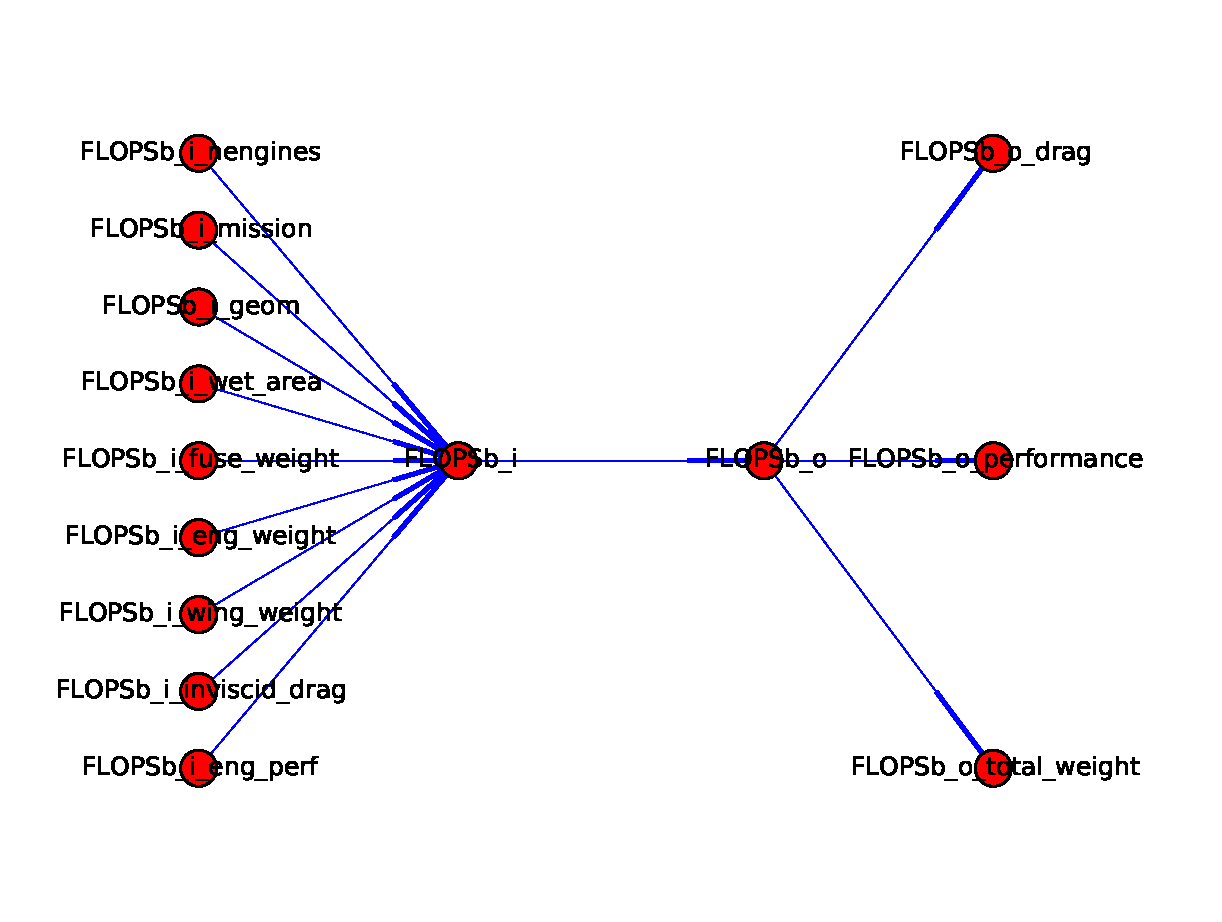
\includegraphics[width=.6\textwidth]{images/FLOPSb_analysis_block}
	  \end{center}
	  \caption{Sample analysis block for analysis code FLOPSb using Table \ref{t:ins and outs}}
	\label{f:FLOPSb analysis block}
	\end{figure}

	\item Variable ((change)) nodes are created to represent the objectives for performance and total weight.

	\item Variable nodes are created to represent the geometry variable and mission variable as global inputs.

	\item Explicit edges are created from each variable node to every other variable node representing variables with the same name. The direction is determined by whether the variable node has an edge directed into or out of a model node (local input or local output).
	\end{enumerate}
	The resulting MCG is shown in Fig.~\ref{f:design vars}. Emerging cycles are shown in yellow and indicate potential cycles that may exist when an FPG is formed.
	\begin{figure}[htb!]
	  \begin{center}
		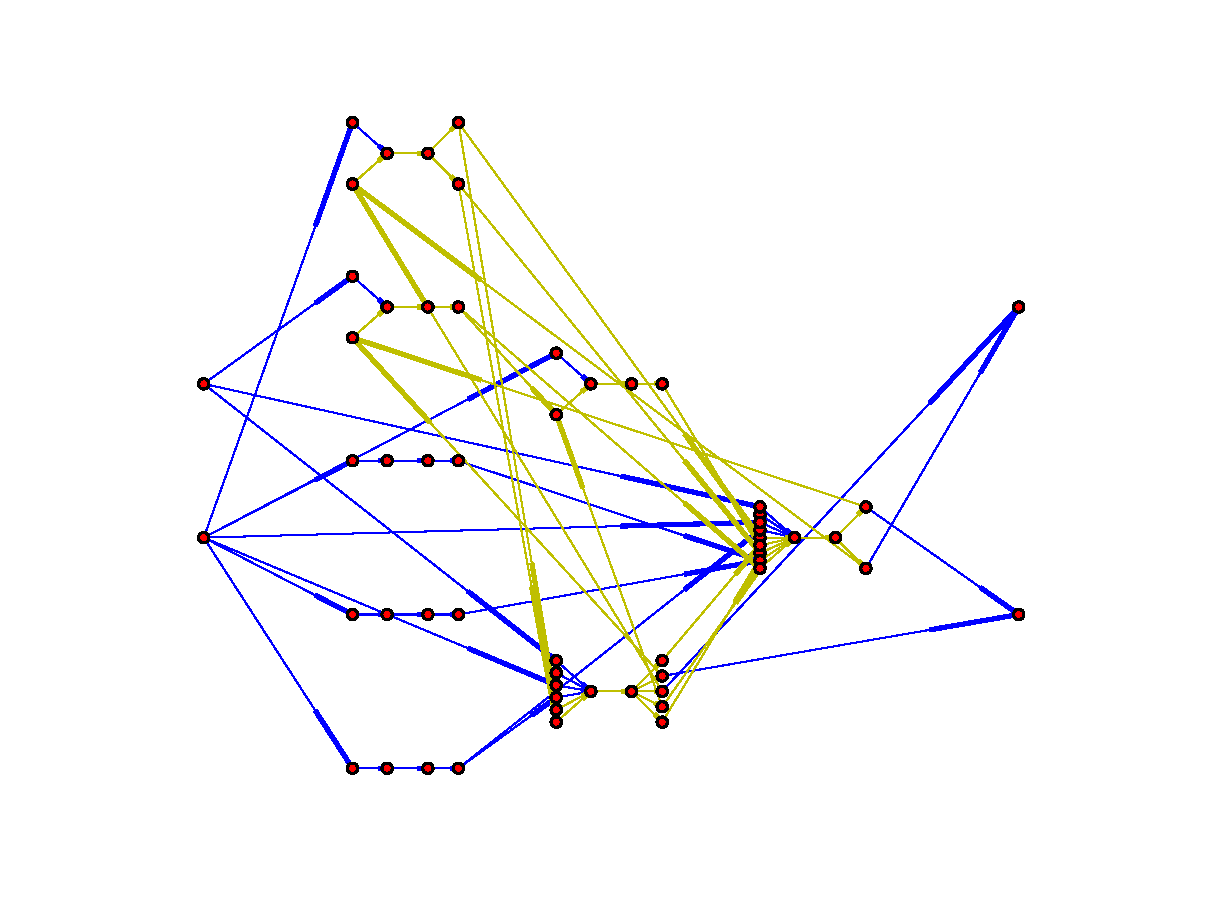
\includegraphics[width=.6\textwidth]{images/MCG}
	  \end{center}
	  \caption{Maximal connectivity graph for the subsonic transport example problem}
	\end{figure}

\subsection{Obtaining an FPG}
	\label{ss:obtaining an FPG}
	The process of obtaining an FPG from the given MCG is expected to be an iterative process in which the user applies the algorithm to determine whether or not an FPG can be obtained, and then modifies the indegree limits or the MCG to obtain a satisfactory FPG. For example, after determining the location of a hole, the user can change the indegree limit to make the node a design variable, or the user could change the MCG by adding a new analysis code such that the hole is resolved.

	As presented in Sec.~\ref{s:building graphs}.\ref{ss:obtaining FPG}, the first step to obtaining an FPG is to detect holes. To start, we set the lower indegree limit for every node to be unity to find any potential holes. In this case, it turns out that the variable nodes representing the number of engines is a hole for NPSS, FLOPSa, and FLOPSb. This implies than an FPG cannot be obtained from the given MCG, as shown in Fig.~\ref{f:MCG nengines}. In this figure, the green nodes indicate analysis blocks with a hole, and the cyan nodes indicate analysis blocks that became unused after the invalid analyses were removed ((connections were removed, color edges too)).
	\begin{figure}[htb!]
	  \begin{center}
		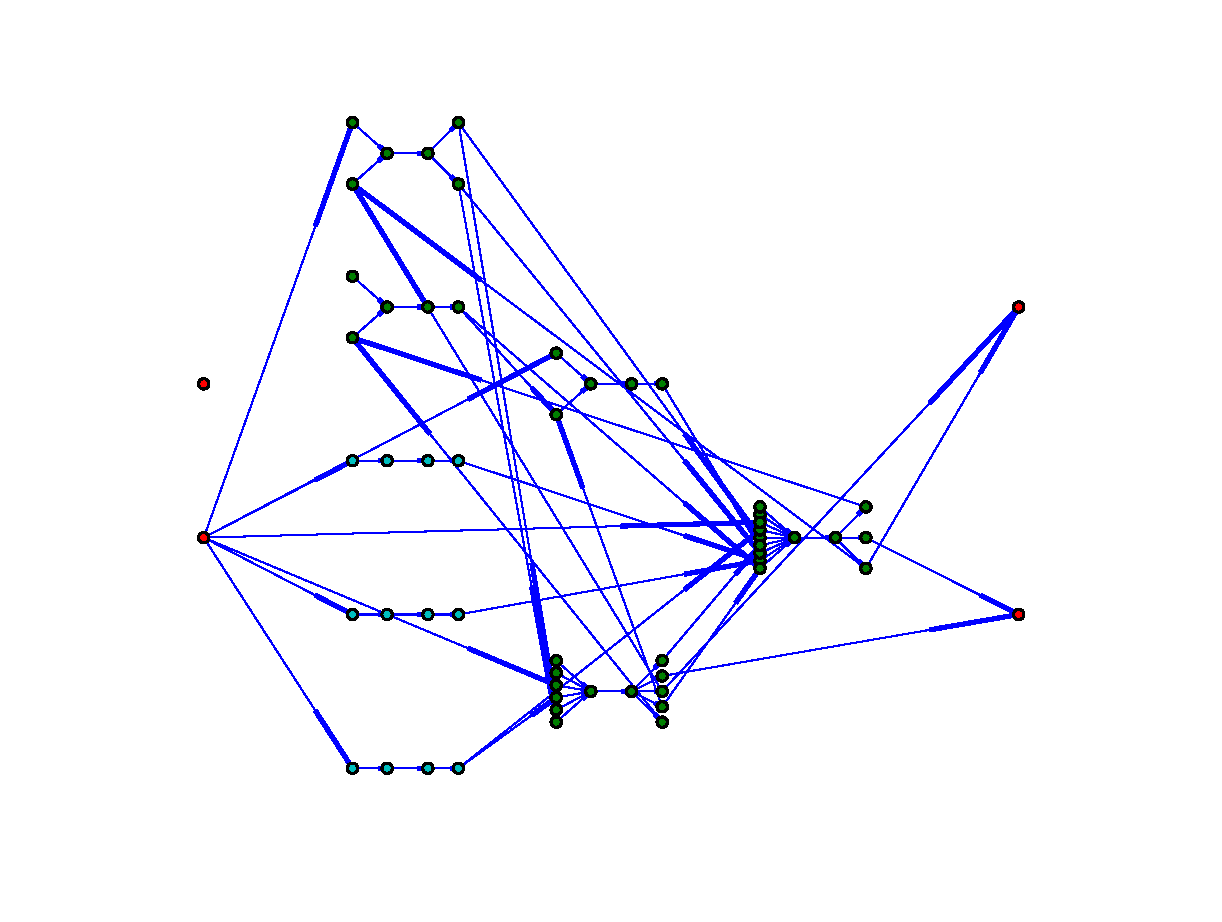
\includegraphics[width=.6\textwidth]{images/MCG_nengines}
	  \end{center}
	  \caption{The MCG with one global variable missing. The resulting holes are shown in green and unused analyses shown in cyan.}
	\label{f:MCG nengines}
	\end{figure}

	Therefore, we may now create another variable node to represent the number of engines as a global input and also create explicit edges to supply this new input. Now this step is repeated with the new MCG and no holes are found.

	While Sec.~\ref{s:building graphs}.\ref{ss:obtaining FPG} indicated the process for obtaining an FPG, it did not specify how to decide which edges to keep when resolving a collision, that freedom is left to the specific implementation. The benefit of this approach is that standard graph theory algorithms can be used to make these decisions. The first example of this is to obtain an FPG with the fewest possible number of cycles, which are found using the implementation of Johnson's algorithm \cite{Johnson1975} in the Python package NetworkX. The FPG with the fewest cycles is shown in Fig.~\ref{f:FPG fewest cycles}, which indicates one cycle shown in yellow. A similar alternative would be to minimize the number of analysis blocks involved in cycles, counting multiplicity.
	\begin{figure}[htb!]
	  \begin{center}
		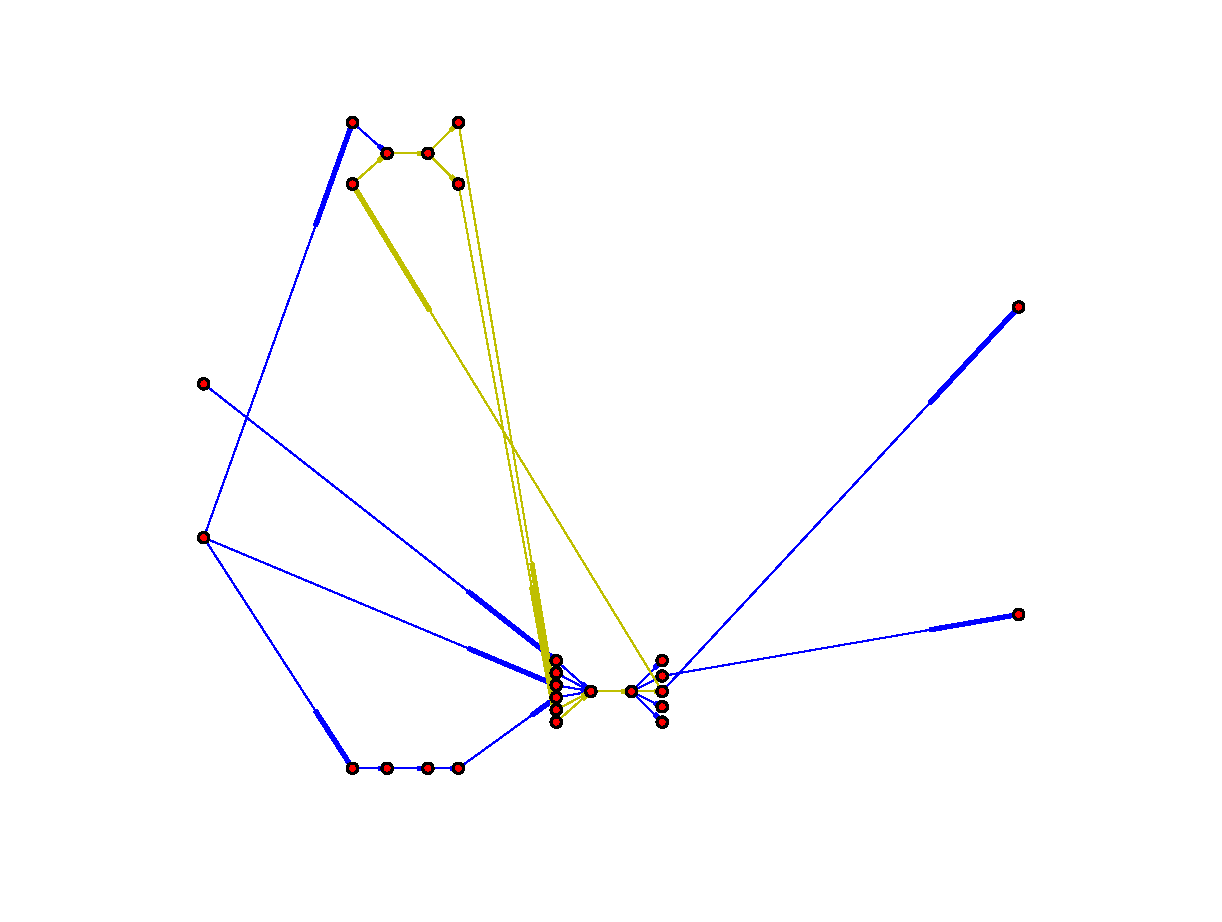
\includegraphics[width=.6\textwidth]{images/FPG_fewest_cycles}
	  \end{center}
	  \caption{FPG with the fewest number of cycles.}
	\label{f:FPG fewest cycles}
	\end{figure}

	Alternatively, it may be desirable to resolving collisions by including the higher fidelity codes, such as NPSS in this case.
	One method to ensure that the edges directed from certain analysis blocks are the ones chosen to resolve the conflicts is to use a ranking system. For this case, consider the rankings for each analysis code given in Table \ref{t:rankings}.
	\begin{table}[htbp]
	  \centering
	  \caption{Example ranking of importance}
		\begin{tabular}{cc}
		\toprule
		analysis code & rank \\
		\midrule
		VSP   & 5 \\
		PDCYL & 5 \\
		NPSS  & 4 \\
		PMARC & 4 \\
		FLOPSb & 4 \\
		VORLAX & 3 \\
		WATE  & 3 \\
		FLOPSa & 2 \\
		\bottomrule
		\end{tabular}%
	  \label{t:rankings}%
	\end{table}% 
	Step two in Sec.~\ref{s:building graphs}.\ref{ss:obtaining FPG} (the resolution of collisions) is now conducted by selecting the edges directed from the analysis blocks with the highest rank for each collision. The resulting FPG is shown in Fig.~\ref{f:FPG highest rank}, and this graph has four cycles, which are enumerated in Table \ref{t:cycles}.
	\begin{figure}[htb!]
	  \begin{center}
		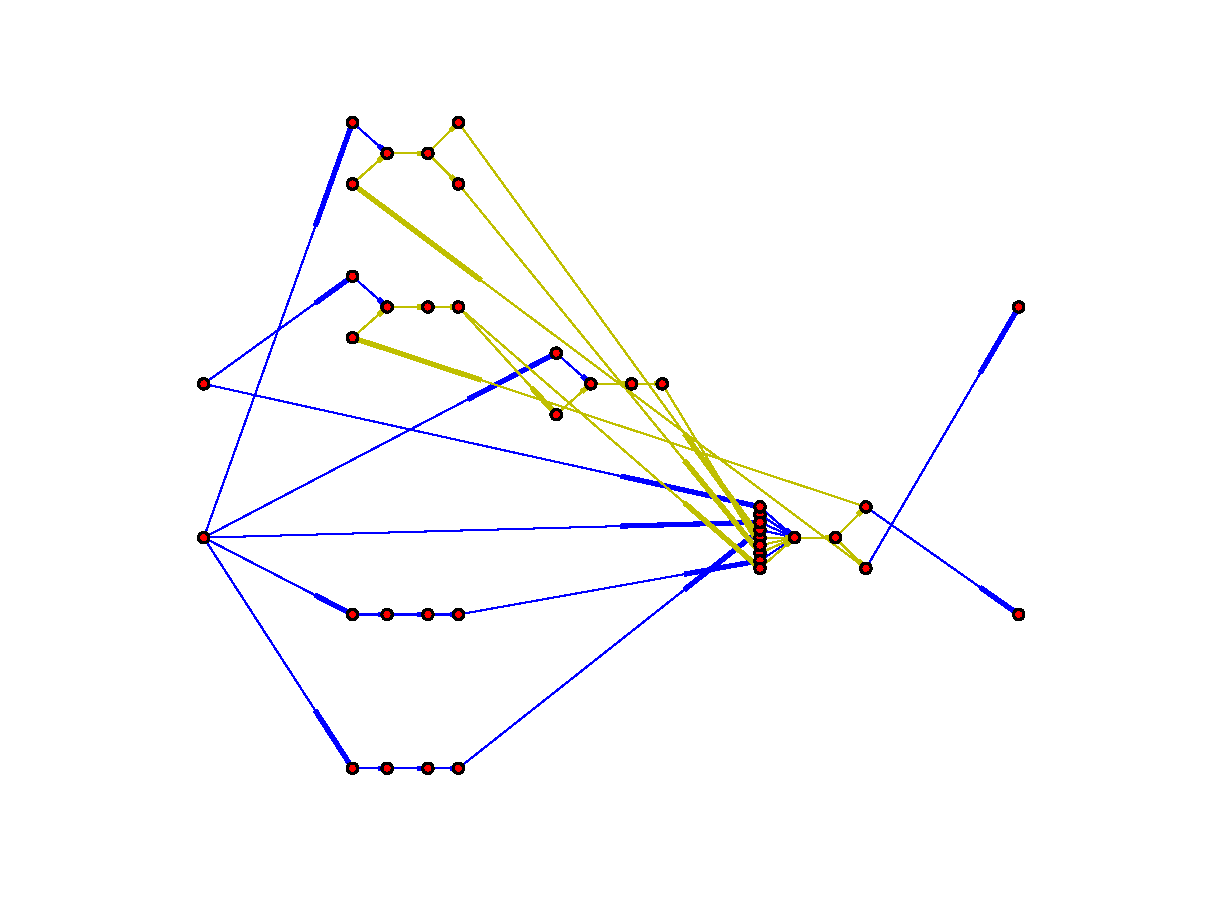
\includegraphics[width=.6\textwidth]{images/FPG_highest_rank}
	  \end{center}
	  \caption{FPG obtained using the ranking system.}
	\label{f:FPG highest rank}
	\end{figure}
	\begin{table}[htbp]
	  \centering
	  \caption{Cycles for the FPG obtained using ranking}
		\begin{tabular}{ccccccc}
		\toprule
		output/input & analysis code & output/input & analysis code & output/input & analysis code & output/input \\
		\midrule
		engine weight & FLOPSb & drag  & NPSS  & engine performance & WATE  & engine weight \\
		engine performance & FLOPSb & drag  & NPSS  & engine performance &       &  \\
		fuselage weight & FLOPSb & total weight & PDCYL & fuselage weight &       &  \\
		wing weight & FLOBSb & total weight & PDCYL & wing weight &       &  \\
		\bottomrule
		\end{tabular}%
	  \label{t:cycles}
	\end{table}%

	Finally, now consider the case where it is desired to have the inviscid drag input into FLOPSb be a multi--fidelity input, meaning that it is sought to use multiple analysis codes to calculate the same variable. This is done simply by setting the upper indegree limit for this node as two and then repreating the (automated) process. In this case, both VORLAX and PMARC are retained, resulting in an FPG that omits only FLOPSa.


%\begin{figure}[htb!]
%  \begin{center}
%    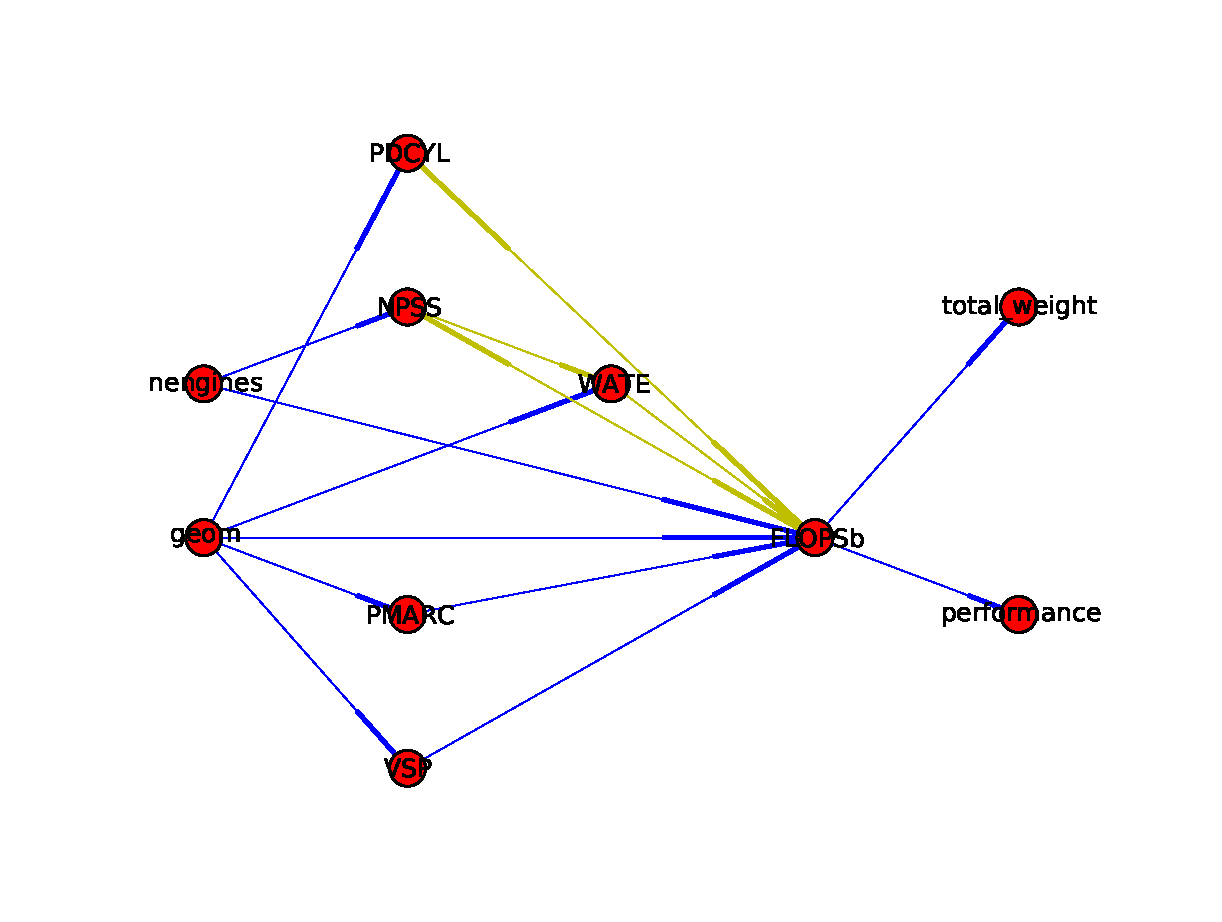
\includegraphics[width=.6\textwidth]{images/FPG_highest_rank_simplified}
%  \end{center}
%  \caption{Simple notional problem with two potential design variables \label{f:design vars}}
%\end{figure}






%\begin{table}[h!]
% \begin{center}
%  \caption{Example problem analysis codes}
%  \label{t:analysis codes}
%  \begin{tabular}{ccc} \hline 
%Analysis code & input variables & output variables \\ \hline
%VSP & geometry & wetted area \\
%PDCYL & geometry & fuselage weight \\
%	& total weight & wing weight \\
%NPSS & number of engines & engine performance \\
%	& drag &	\\
%VORLAX & geometry & inviscid drag \\
%PMARC & geometry & inviscid drag \\
%WATE & geometry & engine weight \\
%	& engine performance &	\\ 
%FLOPSa & number of engines & engine weight \\
%	& mission & performance \\
%	& geometry & total weight \\
%	& wetted area & engine performance \\
%	& fuselage weight & drag \\
%FLOPSb & number of engines & drag \\
%	& mission & performance \\
%	& geometry & total weight \\
%	& wetted area & 	 \\
%	& engine weight & 	\\
%	& wing weight & 	\\
%	& inviscid drag & 	\\
%	& engine performance & 	\\ \hline
%  \end{tabular}
% \end{center}
% \vspace{-15pt}
%\end{table}